\documentclass[9pt,a4paper]{beamer}
\usepackage[utf8]{inputenc}
\usepackage[francais]{babel}
\usepackage[T1]{fontenc}
\usepackage{amsmath}
\usepackage{amsfonts}
\usepackage{amssymb}
\usepackage{makeidx}
\usepackage{graphicx}

\usepackage{color}

\usepackage{listings}

\mode<presentation>

\usetheme{CambridgeUS}

\definecolor{monRouge}{RGB}{204,0,0}
\setbeamercolor{block body alerted}{fg=white,bg=monRouge}

\setbeamertemplate{navigation symbols}{}

\author{\textsc{Frémont} Alexandre et \textsc{Le Calvar} Théo}
\title{Problème des N-Dames}

\begin{document}

\lstdefinestyle{customc}{
  belowcaptionskip=1\baselineskip,
  breaklines=true,
  xleftmargin=\parindent,
  language=C,
  showstringspaces=false,
  basicstyle=\footnotesize\ttfamily,
  keywordstyle=\bfseries\color{green!40!black},
  commentstyle=\itshape\color{purple!40!black},
  identifierstyle=\color{blue},
  stringstyle=\color{orange},
}
\lstset{style=customc}

\begin{frame}
\titlepage
\end{frame}

\begin{frame}
	\frametitle{Plan}
	\tableofcontents
\end{frame}

\section{Introduction}
\begin{frame}

	\begin{block}{Introduction}

	\begin{itemize}
		\item{Probleme N-Dames}

		\item{Les différentes approches}
	\end{itemize}

	\end{block}

\end{frame}

\section{Structure de données}
\begin{frame}[fragile]
	\frametitle{Structure de données}
	\begin{block}{Code}
		\begin{lstlisting}
			typedef struct chessboard {
				size_t          size;
				u32*            queens;
			} cb_t;
		\end{lstlisting}

	\end{block}
\end{frame}

\section{Algorithme CSP}
\begin{frame}
	\frametitle{Algorithmes CSP}

	\begin{block}{Backtracking}
		On construit l'échiquier par étape, lorsque une iteration viole une contrainte on retourne en arrière et on change l'itération.
	\end{block}



	\begin{block}{Forward checking}
		On place nos dames sur l'échiquier et à chaque dame placé on diminue l'espace ou l'on poura placé nos futurs dames \\
		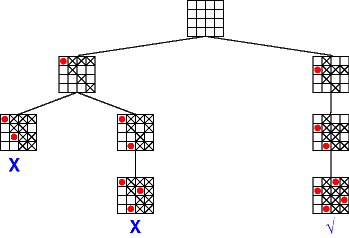
\includegraphics[width=0.4\textwidth]{images/forw.png}
	\end{block}

\end{frame}


\section{Algorithme de recherche local}
\begin{frame}
	\frametitle{Algorithme}

	\begin{block}{1er algorithme de recherche local}
		On dispose les dames sur l'échiquier et on éffectue des transposition entre le dames pour diminué les conflits
	\end{block}

	\begin{block}{2nd algorithme de recherche local}
		On initialise les dames sur l'échiquier de maniere à n'avoir que 100 dames en conflits aux total puis on diminue le nombre de dames en conflit avec des transposition entre elles.
	\end{block}


\end{frame}

\section{Resultat et performance}
\begin{frame}
	\frametitle{Resultat et performance}

	\begin{block}{Backtrack}

	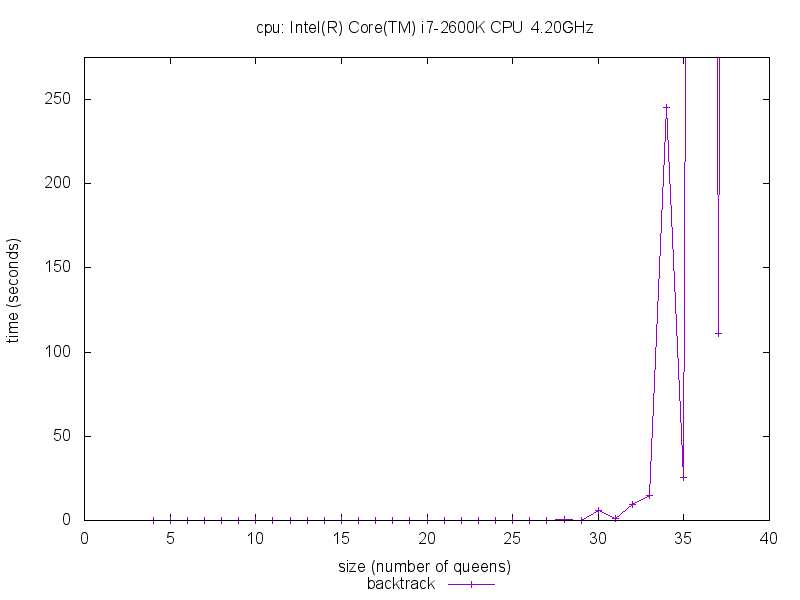
\includegraphics[width=0.3\textwidth]{images/plot_bt_i7.png}

	\end{block}

	\begin{block}{Forward}

	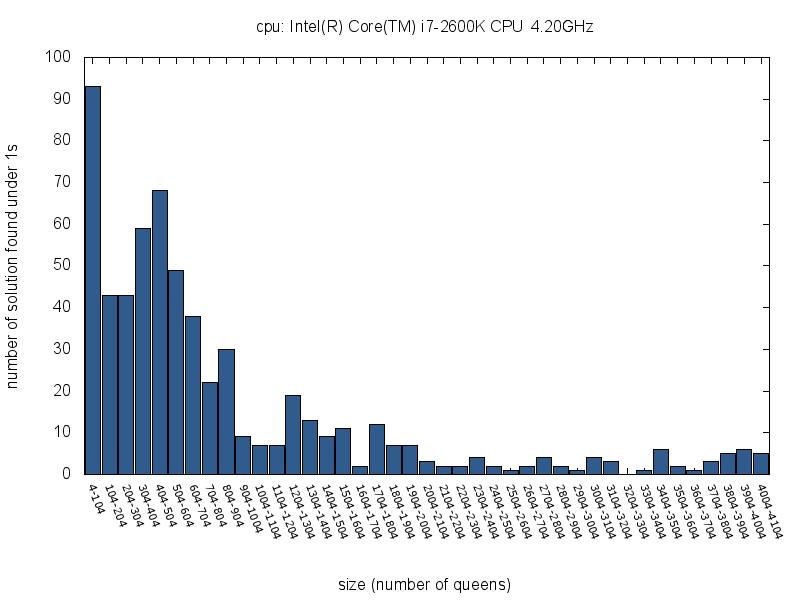
\includegraphics[width=0.3\textwidth]{images/plot_fw_i7.png}

	\end{block}

	\begin{block}{backtrack vs Forward}

	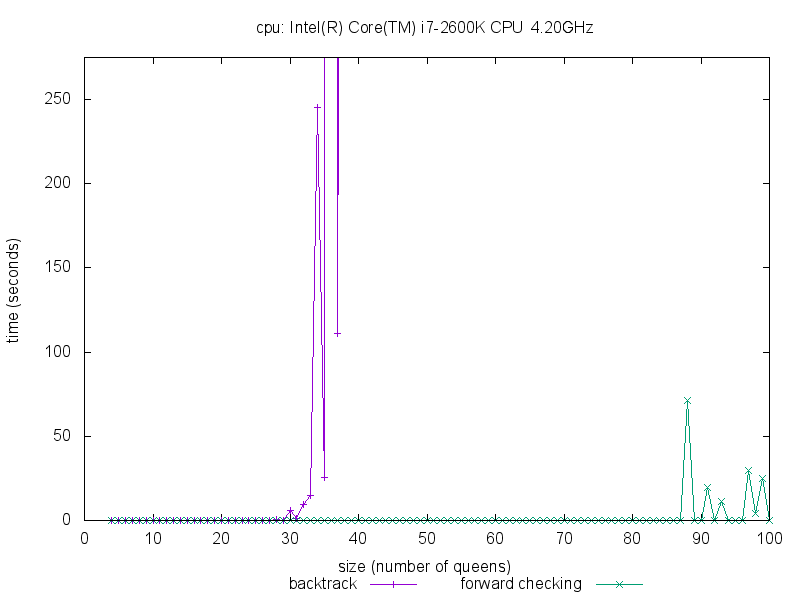
\includegraphics[width=0.3\textwidth]{images/plot_bt_fw_i7.png}

	\end{block}



\end{frame}

\section{Resultat et performance}
\begin{frame}
	\frametitle{Resultat et performance}

	\begin{block}{recherche local}

	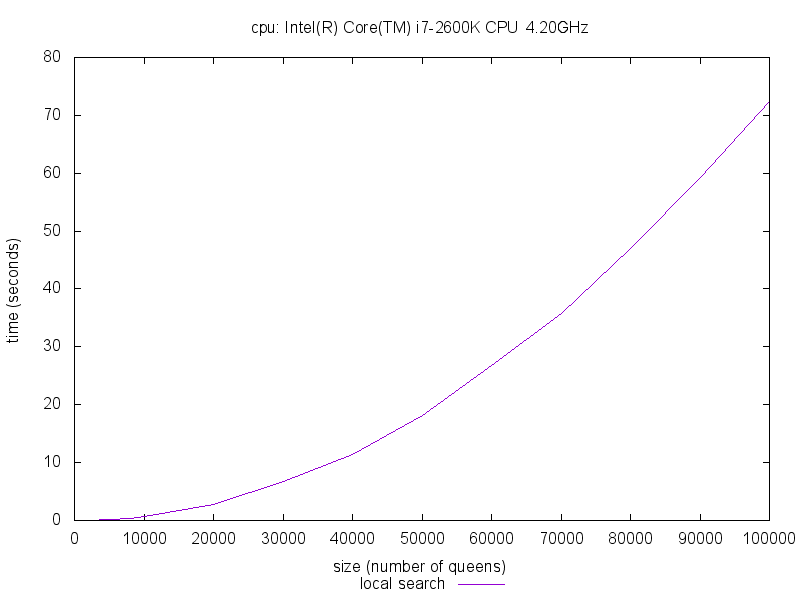
\includegraphics[width=0.3\textwidth]{images/plot_ls_i7.png}

	\end{block}

	\begin{block}{recherche local amélioré}

	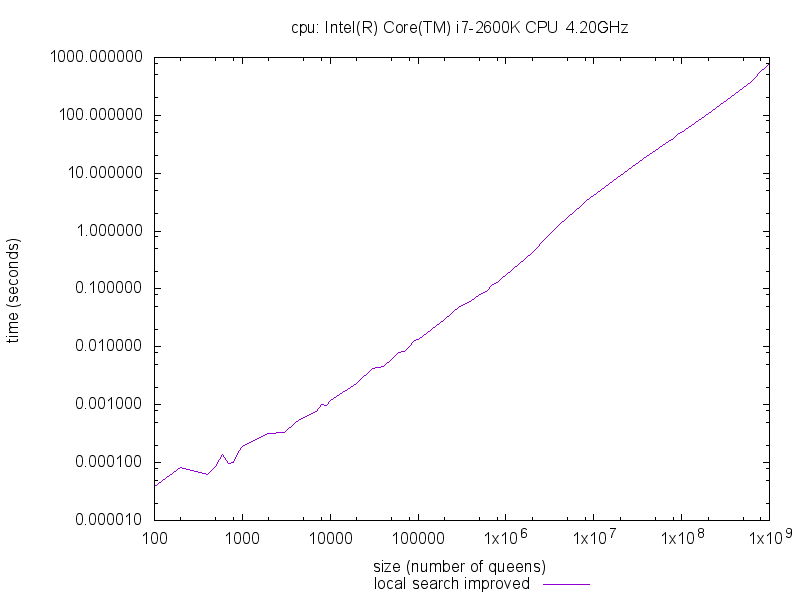
\includegraphics[width=0.3\textwidth]{images/plot_lst_i7.png}

	\end{block}

	\begin{block}{comparaison}

	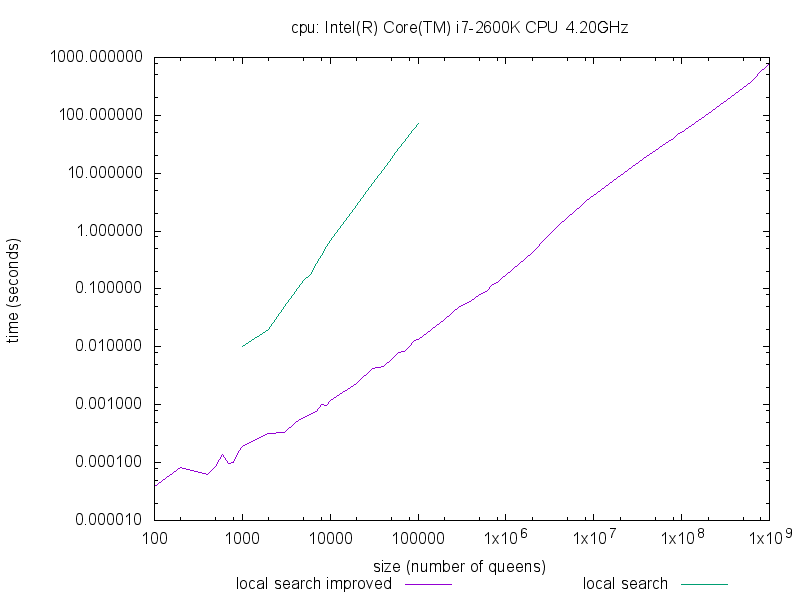
\includegraphics[width=0.3\textwidth]{images/plot_lst_ls_i7.png}

	\end{block}



\end{frame}

\section{Conclusion}
\begin{frame}
	\frametitle{Conclusion}

	\begin{block}{structure de données}


	\end{block}

	\begin{block}{recherche local > Forward}
		Pour finir on remarque que lorsque on veut effectué le problème de n dames sur de grandes instances il faut utilisé de la recherche local.
	\end{block}


\end{frame}


\end{document}
